%! Author = Saeid Yazdani
%! Date = 8/20/2024

\section{Prototyping Approach}
\label{sec:prototyping-approach}

Since the system is a complex design with multiple building blocks, the first
challenge is choosing the most effective solution for realizing the
prototype in terms of time and cost.

Prototyping complex electronic systems requires a method that balances
flexibility, scalability, and ease of modification.

One method is the use of \emph{backplane} and \emph{module cards}, a
strategy that offers a modular approach to system design as shown in
\autoref{fig:backplane-concept}.

\begin{figure}[h!]
    \centering
    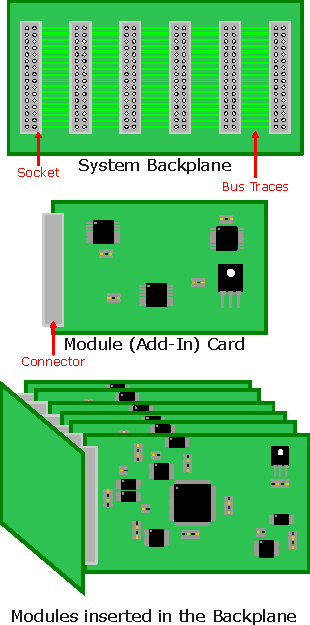
\includegraphics[width=0.5\textwidth]
    {figures/prototype/backplane-add-on-concept}
    \caption[Backplane Concept]{The concept of backplane and module cards.}
    \label{fig:backplane-concept}
\end{figure}

Add-in cards are modular circuit boards that perform specific functions within
the system. Each card is designed to handle a particular task, such as
processing, input/output interfacing, power management, or communication.
By plugging into the backplane, these cards contribute to the system's overall
functionality.

While the entirety of the system may be designed in one large \ac{PCB} as
it will be a more cost-effective approach for mass production if the design
is well proven, the backplane-based approach
allows independent development of system modules with the following
benefits:

\begin{itemize}[topsep=8pt,itemsep=4pt,partopsep=4pt, parsep=4pt]

    \item \textbf{Rapid Prototyping:} Each module can be designed and
    produced independently.
    If there are any problems found post-production, they will be
    limited to that particular module and only that module needs to
    undergo re-design and re-production.

    \item \textbf{Ease of Evaluating:} Designers can test various configurations
    by swapping in and out modules from the backplane to explore different
    possibilities without the need for rework.

\end{itemize}

Resorting to backplane and module cards has its unique challenges that
can affect the overall performance of the system under development
in terms of signal integrity and maximum performance. Possible drawbacks
of backplanes are:

\begin{itemize}[topsep=8pt,itemsep=4pt,partopsep=4pt, parsep=4pt]
    \item \textbf{Long Trace Lengths:}
    The physical distance between add-in cards in the backplane can lead to
    longer trace lengths, which may cause signal degradation and increased
    latency, especially in systems where data must traverse multiple stages or
    if the bus is shared amongst many devices.
    This could be problematic in time-sensitive applications where fast
    response times are critical.

    \item \textbf{Crosstalk and \acs{EMI}:}
    Tightly spaced traces on the backplane can lead to crosstalk, where signals
    on one trace interfere with those on adjacent traces.
    High-frequency signals can generate electromagnetic interference and
    potentially limit the performance or cause corruption of data.

    \item \textbf{Thermal Management:}
    Densely packed add-in cards can generate significant heat.

    \item \textbf{Mechanical Stability:}
    Unstable and loose connections between modules and backplane can lead to
    intermittent failures.

\end{itemize}
